\addcontentsline{toc}{section}{Appendix} % Remove this if you don't want the appendix included in the table of contents.
\appendix

\section{MATLAB Code}\label{sec:matlab}
This section should contain your MATLAB code. DO NOT attach files posted online (that you didn't write). Note that the method used to input code below does not look as pretty when the lines are too long.

\subsection{plot\_constraint.m}\label{sec:plot_constraint_m}
\lstinputlisting{code/plot_constraint.m}\section{Simulink Diagrams}\label{sec:simulink}
This section should contain your Simulink diagrams. Just like the plots, these should be in vector format, like in \Cref{fig:simulink}. Make them tidy enough to understand.

\subsection{Simulink Diagrams for Part II}
\begin{figure}[!!ht!!!!!!!!tb!!]
    	\centering
		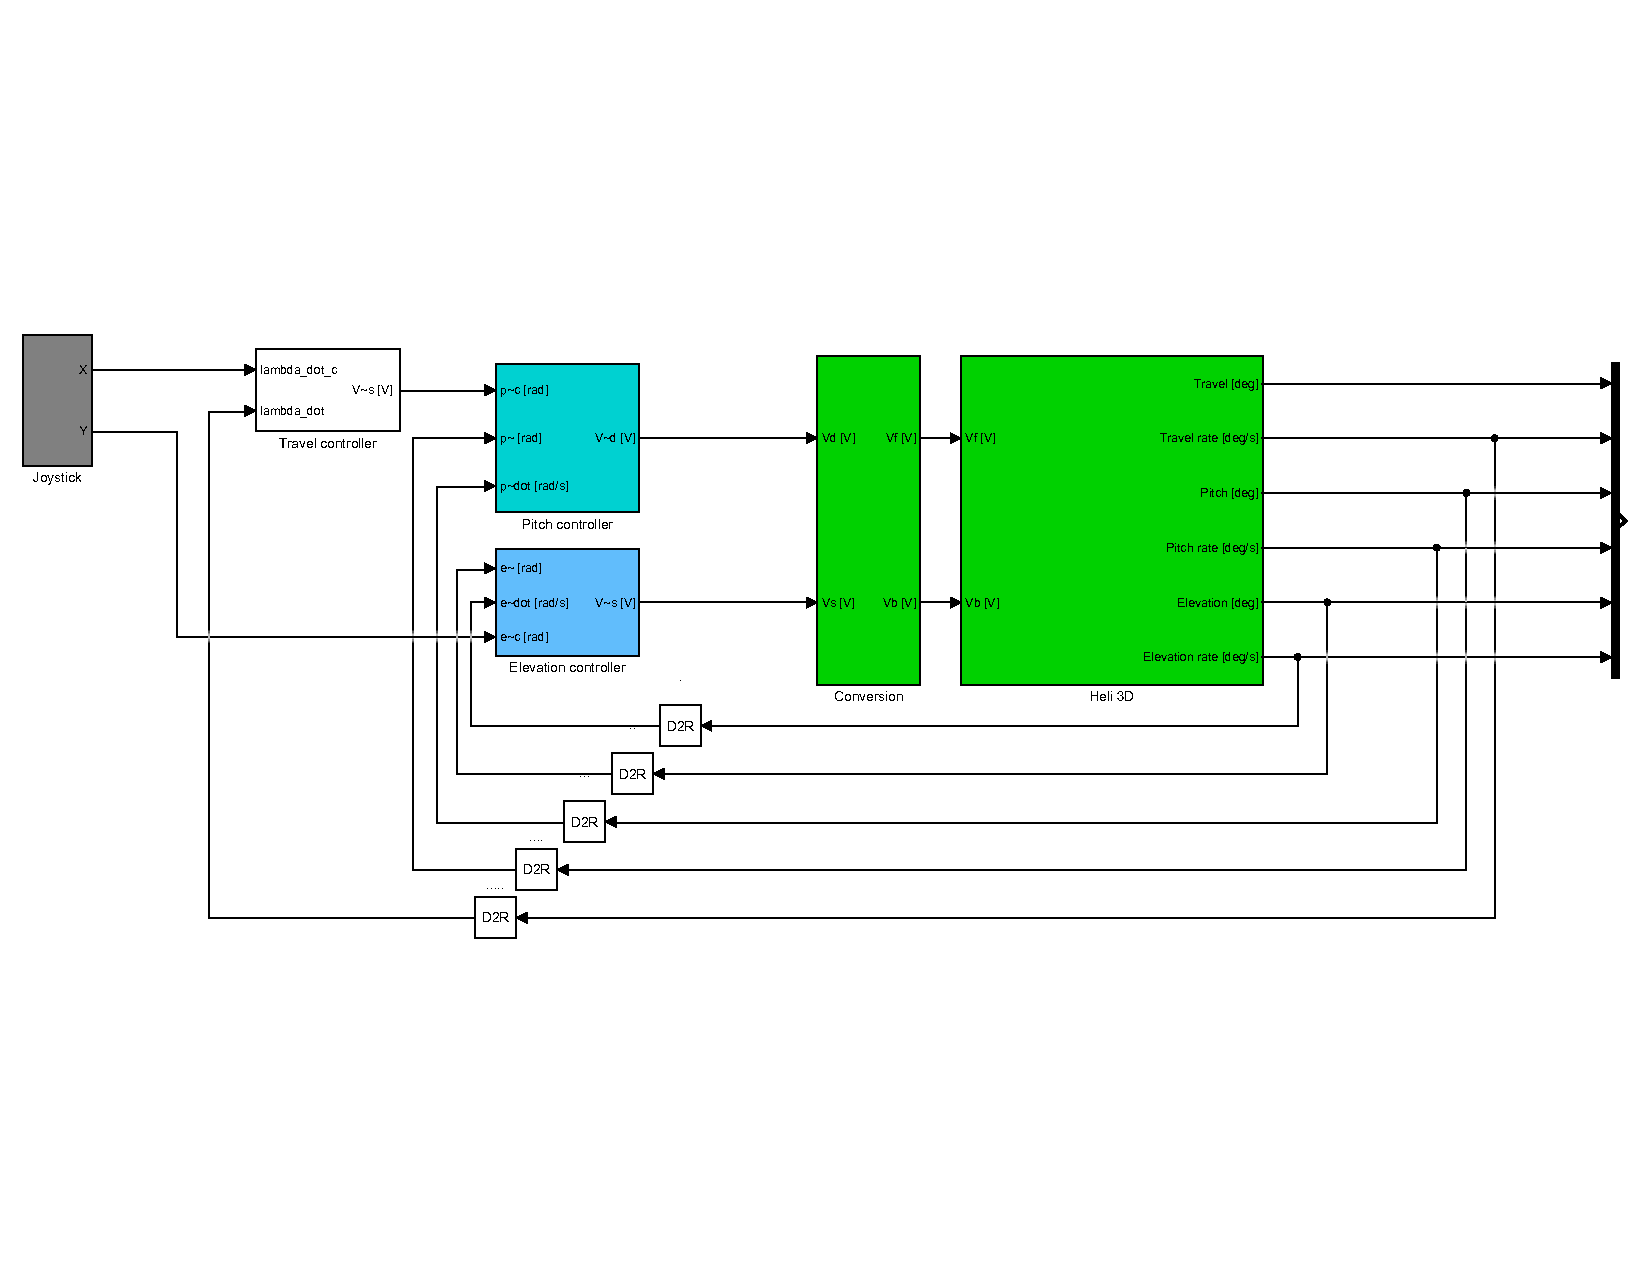
\includegraphics[width=1.1\textwidth,trim={0cm 3cm 0cm 5cm},clip]{figures/simulink/P2p2.pdf}
    	\caption{Top view of model from Part 2 problem 2}
\label{fig:P2p2_simulink}
\end{figure}
\FloatBarrier

\section{Parameters and values}\label{sec:parameters}


\begin{table}[tbp]
	\centering
	\caption{Parameters and values.}
	\begin{tabular}{llll}
		\toprule
		Symbol & Parameter & Value & Unit \\
		\midrule
		$l_h$ & Distance from elevation axis to helicopter body & $0.63$  & \meter                      \\
		$l_p$ & Distance from pitch axis to motor               & $0.18$  & \meter                      \\
		$K_f$ & Force constant motor                            & $0.25$  & \newton\per\volt            \\
		$J_e$ & Moment of inertia for elevation                 & $0.83$  & \kilogram\usk\meter\squared \\
$J_{\lambda}$ & Moment of inertia for travel                    & $0.83$  & \kilogram\usk\meter\squared \\
		$J_p$ & Moment of inertia for pitch                     & $0.034$ & \kilogram\usk\meter\squared \\
		$m_p$ & Mass of helicopter                              & $1.05$  & \kilogram                   \\
		$m_c$ & Weight of counterweight                         & $1.87$  & \kilogram                   \\
		\bottomrule
	\end{tabular}
\label{tab:parameters}
\end{table}
